% Options for packages loaded elsewhere
% Options for packages loaded elsewhere
\PassOptionsToPackage{unicode}{hyperref}
\PassOptionsToPackage{hyphens}{url}
\PassOptionsToPackage{dvipsnames,svgnames,x11names}{xcolor}
%
\documentclass[
  11pt,
  letterpaper,
  DIV=11,
  numbers=noendperiod]{scrartcl}
\usepackage{xcolor}
\usepackage{amsmath,amssymb}
\setcounter{secnumdepth}{5}
\usepackage{iftex}
\ifPDFTeX
  \usepackage[T1]{fontenc}
  \usepackage[utf8]{inputenc}
  \usepackage{textcomp} % provide euro and other symbols
\else % if luatex or xetex
  \usepackage{unicode-math} % this also loads fontspec
  \defaultfontfeatures{Scale=MatchLowercase}
  \defaultfontfeatures[\rmfamily]{Ligatures=TeX,Scale=1}
\fi
\usepackage{lmodern}
\ifPDFTeX\else
  % xetex/luatex font selection
\fi
% Use upquote if available, for straight quotes in verbatim environments
\IfFileExists{upquote.sty}{\usepackage{upquote}}{}
\IfFileExists{microtype.sty}{% use microtype if available
  \usepackage[]{microtype}
  \UseMicrotypeSet[protrusion]{basicmath} % disable protrusion for tt fonts
}{}
% Make \paragraph and \subparagraph free-standing
\makeatletter
\ifx\paragraph\undefined\else
  \let\oldparagraph\paragraph
  \renewcommand{\paragraph}{
    \@ifstar
      \xxxParagraphStar
      \xxxParagraphNoStar
  }
  \newcommand{\xxxParagraphStar}[1]{\oldparagraph*{#1}\mbox{}}
  \newcommand{\xxxParagraphNoStar}[1]{\oldparagraph{#1}\mbox{}}
\fi
\ifx\subparagraph\undefined\else
  \let\oldsubparagraph\subparagraph
  \renewcommand{\subparagraph}{
    \@ifstar
      \xxxSubParagraphStar
      \xxxSubParagraphNoStar
  }
  \newcommand{\xxxSubParagraphStar}[1]{\oldsubparagraph*{#1}\mbox{}}
  \newcommand{\xxxSubParagraphNoStar}[1]{\oldsubparagraph{#1}\mbox{}}
\fi
\makeatother


\usepackage{longtable,booktabs,array}
\usepackage{calc} % for calculating minipage widths
% Correct order of tables after \paragraph or \subparagraph
\usepackage{etoolbox}
\makeatletter
\patchcmd\longtable{\par}{\if@noskipsec\mbox{}\fi\par}{}{}
\makeatother
% Allow footnotes in longtable head/foot
\IfFileExists{footnotehyper.sty}{\usepackage{footnotehyper}}{\usepackage{footnote}}
\makesavenoteenv{longtable}
\usepackage{graphicx}
\makeatletter
\newsavebox\pandoc@box
\newcommand*\pandocbounded[1]{% scales image to fit in text height/width
  \sbox\pandoc@box{#1}%
  \Gscale@div\@tempa{\textheight}{\dimexpr\ht\pandoc@box+\dp\pandoc@box\relax}%
  \Gscale@div\@tempb{\linewidth}{\wd\pandoc@box}%
  \ifdim\@tempb\p@<\@tempa\p@\let\@tempa\@tempb\fi% select the smaller of both
  \ifdim\@tempa\p@<\p@\scalebox{\@tempa}{\usebox\pandoc@box}%
  \else\usebox{\pandoc@box}%
  \fi%
}
% Set default figure placement to htbp
\def\fps@figure{htbp}
\makeatother


% definitions for citeproc citations
\NewDocumentCommand\citeproctext{}{}
\NewDocumentCommand\citeproc{mm}{%
  \begingroup\def\citeproctext{#2}\cite{#1}\endgroup}
\makeatletter
 % allow citations to break across lines
 \let\@cite@ofmt\@firstofone
 % avoid brackets around text for \cite:
 \def\@biblabel#1{}
 \def\@cite#1#2{{#1\if@tempswa , #2\fi}}
\makeatother
\newlength{\cslhangindent}
\setlength{\cslhangindent}{1.5em}
\newlength{\csllabelwidth}
\setlength{\csllabelwidth}{3em}
\newenvironment{CSLReferences}[2] % #1 hanging-indent, #2 entry-spacing
 {\begin{list}{}{%
  \setlength{\itemindent}{0pt}
  \setlength{\leftmargin}{0pt}
  \setlength{\parsep}{0pt}
  % turn on hanging indent if param 1 is 1
  \ifodd #1
   \setlength{\leftmargin}{\cslhangindent}
   \setlength{\itemindent}{-1\cslhangindent}
  \fi
  % set entry spacing
  \setlength{\itemsep}{#2\baselineskip}}}
 {\end{list}}
\usepackage{calc}
\newcommand{\CSLBlock}[1]{\hfill\break\parbox[t]{\linewidth}{\strut\ignorespaces#1\strut}}
\newcommand{\CSLLeftMargin}[1]{\parbox[t]{\csllabelwidth}{\strut#1\strut}}
\newcommand{\CSLRightInline}[1]{\parbox[t]{\linewidth - \csllabelwidth}{\strut#1\strut}}
\newcommand{\CSLIndent}[1]{\hspace{\cslhangindent}#1}



\setlength{\emergencystretch}{3em} % prevent overfull lines

\providecommand{\tightlist}{%
  \setlength{\itemsep}{0pt}\setlength{\parskip}{0pt}}



 


\usepackage{caption}
\captionsetup{font=small, labelfont=bf}
\setlength{\parindent}{0pt}
\setlength{\parskip}{1.25ex}
\KOMAoption{captions}{tableheading}
\makeatletter
\@ifpackageloaded{caption}{}{\usepackage{caption}}
\AtBeginDocument{%
\ifdefined\contentsname
  \renewcommand*\contentsname{Table of contents}
\else
  \newcommand\contentsname{Table of contents}
\fi
\ifdefined\listfigurename
  \renewcommand*\listfigurename{List of Figures}
\else
  \newcommand\listfigurename{List of Figures}
\fi
\ifdefined\listtablename
  \renewcommand*\listtablename{List of Tables}
\else
  \newcommand\listtablename{List of Tables}
\fi
\ifdefined\figurename
  \renewcommand*\figurename{Figure}
\else
  \newcommand\figurename{Figure}
\fi
\ifdefined\tablename
  \renewcommand*\tablename{Table}
\else
  \newcommand\tablename{Table}
\fi
}
\@ifpackageloaded{float}{}{\usepackage{float}}
\floatstyle{ruled}
\@ifundefined{c@chapter}{\newfloat{codelisting}{h}{lop}}{\newfloat{codelisting}{h}{lop}[chapter]}
\floatname{codelisting}{Listing}
\newcommand*\listoflistings{\listof{codelisting}{List of Listings}}
\makeatother
\makeatletter
\makeatother
\makeatletter
\@ifpackageloaded{caption}{}{\usepackage{caption}}
\@ifpackageloaded{subcaption}{}{\usepackage{subcaption}}
\makeatother
\usepackage{bookmark}
\IfFileExists{xurl.sty}{\usepackage{xurl}}{} % add URL line breaks if available
\urlstyle{same}
\hypersetup{
  pdftitle={Texture family processing between regions of the visual cortex},
  pdfauthor={Al Xin},
  colorlinks=true,
  linkcolor={blue},
  filecolor={Maroon},
  citecolor={Blue},
  urlcolor={Blue},
  pdfcreator={LaTeX via pandoc}}


\title{Texture family processing between regions of the visual cortex}
\author{\small Al Xin}
\date{Jul 8, 2026}
\begin{document}
\maketitle


\section{Introduction}\label{introduction}

In my ADA, I am analyzing data provided by Gerick Lee et al.~(2024)
containing longitudinal and inter-region neural responses to visual
texture stimuli (available on
\href{https://zenodo.org/records/10888270}{Zenodo})
{[}\citeproc{ref-lee_developmentally_2024}{1}{]}. Lee et al.~recorded
from 6 macaques with two arrays each, targeting V1, V2, V4, and IT.

My goal is to characterize encoding differences between texture groups
between regions, where groups are unique coherence-family combinations
(70 groups), i.e., samples with similar visual statistics. Ziemba et
al.~(2016) performed a similar analysis on recordings from V1 and V2
{[}\citeproc{ref-ziemba_selectivity_2016}{2}{]}, discussed further in
Section~\ref{sec-lit}. Relatedly, Okazawa et al.~(2015, 2017) compared
the selectivity of V2 and V4 neurons for image statistics in texture
stimuli
{[}\citeproc{ref-okazawa_image_2015}{3},\citeproc{ref-okazawa_gradual_2017}{4}{]}.
Other analyses of between-region texture responses focused on
discrimination between noisy and naturalistic structure or selectivity
for natural structure
{[}\citeproc{ref-lee_developmentally_2024}{1},\citeproc{ref-freeman_functional_2013}{5},\citeproc{ref-lee_emergence_2025}{6}{]},
generally finding better discrimination of coherence in V2 and V4.

We expect to find better between-group discrimination in V2 and V4,
consistent with previous work characterizing selectivity to
noisy/naturalistic structure in these brain regions. Furthermore, we
also expect better within-group discrimination in V1, i.e., more
separation between unique samples with the same visual statistics. That
is, later visual regions better encode relevant group-level visual
statistics at the cost of distinctively encoding individual instances of
textures with the same statistics.

\subsection{Notes}\label{notes}

\begin{itemize}
\tightlist
\item
  Consecutive question marks (??) tag areas to follow up on.
\item
  Though the Lee et al.~paper and related literature describes textures
  without V1-like correlations as ``noise'', I often use the term
  ``noisy''.
\item
  Unless otherwise specificed, \(d'\) is Cohon's \(d\), i.e.,
  \(d' = \frac{\mu_1 - \mu_0}{\sqrt{(\sigma^2_1 + \sigma^2_0)/2}}\).
\item
  The published data only includes multi-unit activations (MUAs) for
  each recording site, but I may refer to these as neurons or cells.
\item
  Section~\ref{sec-data} mostly copies information from the previous
  report.
\end{itemize}

\section{Analysis plan}\label{analysis-plan}

For a simple analysis, I plan to calculate the \(d'\) between all group
pairs (i.e., \(\binom{70}{2} = 2415\) pairs per region) and the
one-vs-rest \(d'\) for all individual sites. For the within-family
spread, I could calculate the pairwise or one-vs-rest \(d'\) again, or
perform a nested ANOVA analysis (used in
{[}\citeproc{ref-ziemba_selectivity_2016}{2}{]}). I do not have a
concrete plan for quantifying the between-region differences from these
distances; I'll start with a histogram to visualize it. Dimensionality
reduction techniques like PCA or t-SNE (used in
{[}\citeproc{ref-ziemba_selectivity_2016}{2}{]}) could also help
visualize the data structure and identify clustering.

For population analyses, obstacles include identifying reliable sites
and correcting for different population sizes between regions. Prior
work by Lee et al.~(2024, 2025) applied population decoding techniques
to characterize noisy/naturalistic discriminability
{[}\citeproc{ref-lee_developmentally_2024}{1},\citeproc{ref-lee_emergence_2025}{6}{]}.
To find visually responsive (reliable) sites, Lee et al.~averaged the
site response within samples with the same image statistics (so
\(35 \times 2\) coherence-family combinations plus one element for
blank) then kept sites with a correlation of \(\rho \geq 0.4\) between
even and odd repetitions. They accounted for different population sizes
by repeatedly subsampling sites. See Section~\ref{sec-lit} for the
procedure to calculate the population \(d'\).

Another likely difficulty will be detecting any signal in IT recordings,
and I may need to consider other techniques to characterize IT (e.g.,
manifold learning). Though if nothing shows up with simpler techniques,
I suspect it would be due to the quality of the data rather than the
method.

\section{Prior work}\label{sec-lit}

At AREADNE 2024, Gerick presented a poster covering some family
discrimination results on this data. They ``measured population
distances between different texture families (noise vs.~noise, or
naturalistic vs.~naturalistic), using the same population decoder'',
with results of pairwise comparisons in Figure~\ref{fig-areadne2024}.
Lee et al.~trained the population decoder by:

\begin{enumerate}
\def\labelenumi{\arabic{enumi}.}
\tightlist
\item
  Taking a training set of repetitions (15-fold CV separated by sample).
\item
  Projecting the population response to non-blank images onto the first
  several principal components. Gerick mentioned this step was omitted
  in later analyses. Performing LDA on the original data works fine.
\item
  Applying linear discriminant analysis (LDA) to find the axis
  separating the naturalistic and noisy textures. For between-family
  discrimination, this is replaced by finding the axis best separating
  the families.
\item
  Projecting held-out responses on the axis, then reporting the \(d'\)
  on the resulting values.
\end{enumerate}

\begin{figure}

\centering{

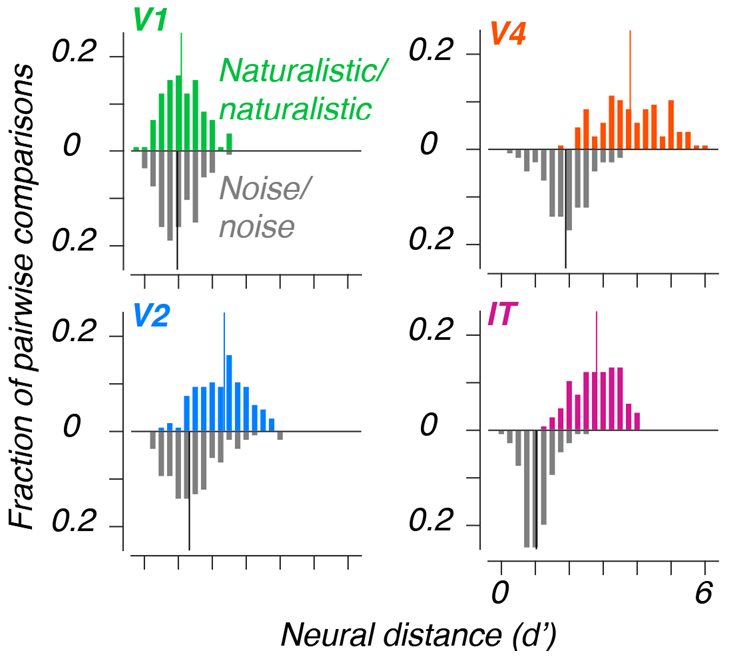
\includegraphics[width=0.4\linewidth,height=\textheight,keepaspectratio]{../img/lee2024-poster-1.png}

}

\caption{\label{fig-areadne2024}Histograms of pairwise comparisons, for
naturalistic-naturalistic comparisons (colored bars), and noise-noise
comparisons (gray). Lines depict medians.}

\end{figure}%

I will be using Gerick's work as a template for my population analysis
approach, though I would also include naturalistic vs.~noisy family
comparisons.

As mentioned above, this ADA direction is similar to Ziemba et
al.~(2016), though their experiment did not include noisy texture
stimuli or recordings from V4/IT
{[}\citeproc{ref-ziemba_selectivity_2016}{2}{]}. They found the
following result:

\begin{quote}
For populations of up to 100 cells, V1 neurons supported better
performance in the sample identification task, whereas V2 neurons
exhibited better performance in texture classification. Relative to V1,
the responses of V2 show greater selectivity and tolerance for the
representation of texture statistics.
\end{quote}

Ziemba et al.~(2016) performed a nested ANOVA to partition response
variance into between-family, within-family, and within-image
(repetition) contributions. Ziemba et al.~(2016) also compared the
performance of a Poisson decoder on classifying samples or families,
though their data contained the same number of families and samples
within families (15 families, 15 samples). This might be viable, but I
would need to subsample groups to make the classification results
comparable.

\section{Data}\label{sec-data}

Monkeys were presented with textures generated from the PS parametric
texture model {[}\citeproc{ref-portilla_parametric_2000}{7}{]}, with
unique images created from 2 levels of coherence (noisy/naturalistic),
35 families (seed images), and 15 randomly generated samples from each
family (1050 unique images) Each region (V1, V2, V4, IT) has at least
one 96 electrode array with data as multi-unit activations. There are
six repetitions of each image per session.

\subsection{Texture stimuli from the PS
model}\label{texture-stimuli-from-the-ps-model}

Textures were generated from the Portilla and Simoncelli (PS) parametric
texture model, a multilevel generative model that produces sample images
by matching visual statistics to an original seed image
{[}\citeproc{ref-portilla_parametric_2000}{7}{]}. The lowest level of
the model matches the local statistic of the original image, e.g., the
correlation in luminance between adjacent pixels, the average luminance
in a small area, or the total variation in luminance. Subsequent layers
control higher level correlations, e.g., correlations between
neighboring patterns of pixels.

Portilla and Simoncelli describe the higher levels as V1-like, or
analogous to the receptive fields of the primary visual cortex. Matching
V1-like correlations produces more coherent \emph{naturalistic}
structure. Example noisy and naturalistic images can be seen in
Figure~\ref{fig-textures} (left). Though the degree of naturalistic
structure varied in the behavioral task, the passive fixation recordings
only contained noisy/zero strength textures or full strength
naturalistic textures. Lee et al.~generated 15 samples of noisy and
naturalistic images from 35 families (\(15 \times 35 \times 2\) unique
images), where each family corresponded to a different original seed
image. The parameters fed into the PS model are likely lost, but the
images presented to the monkeys may be available (??).

\begin{figure}

\centering{

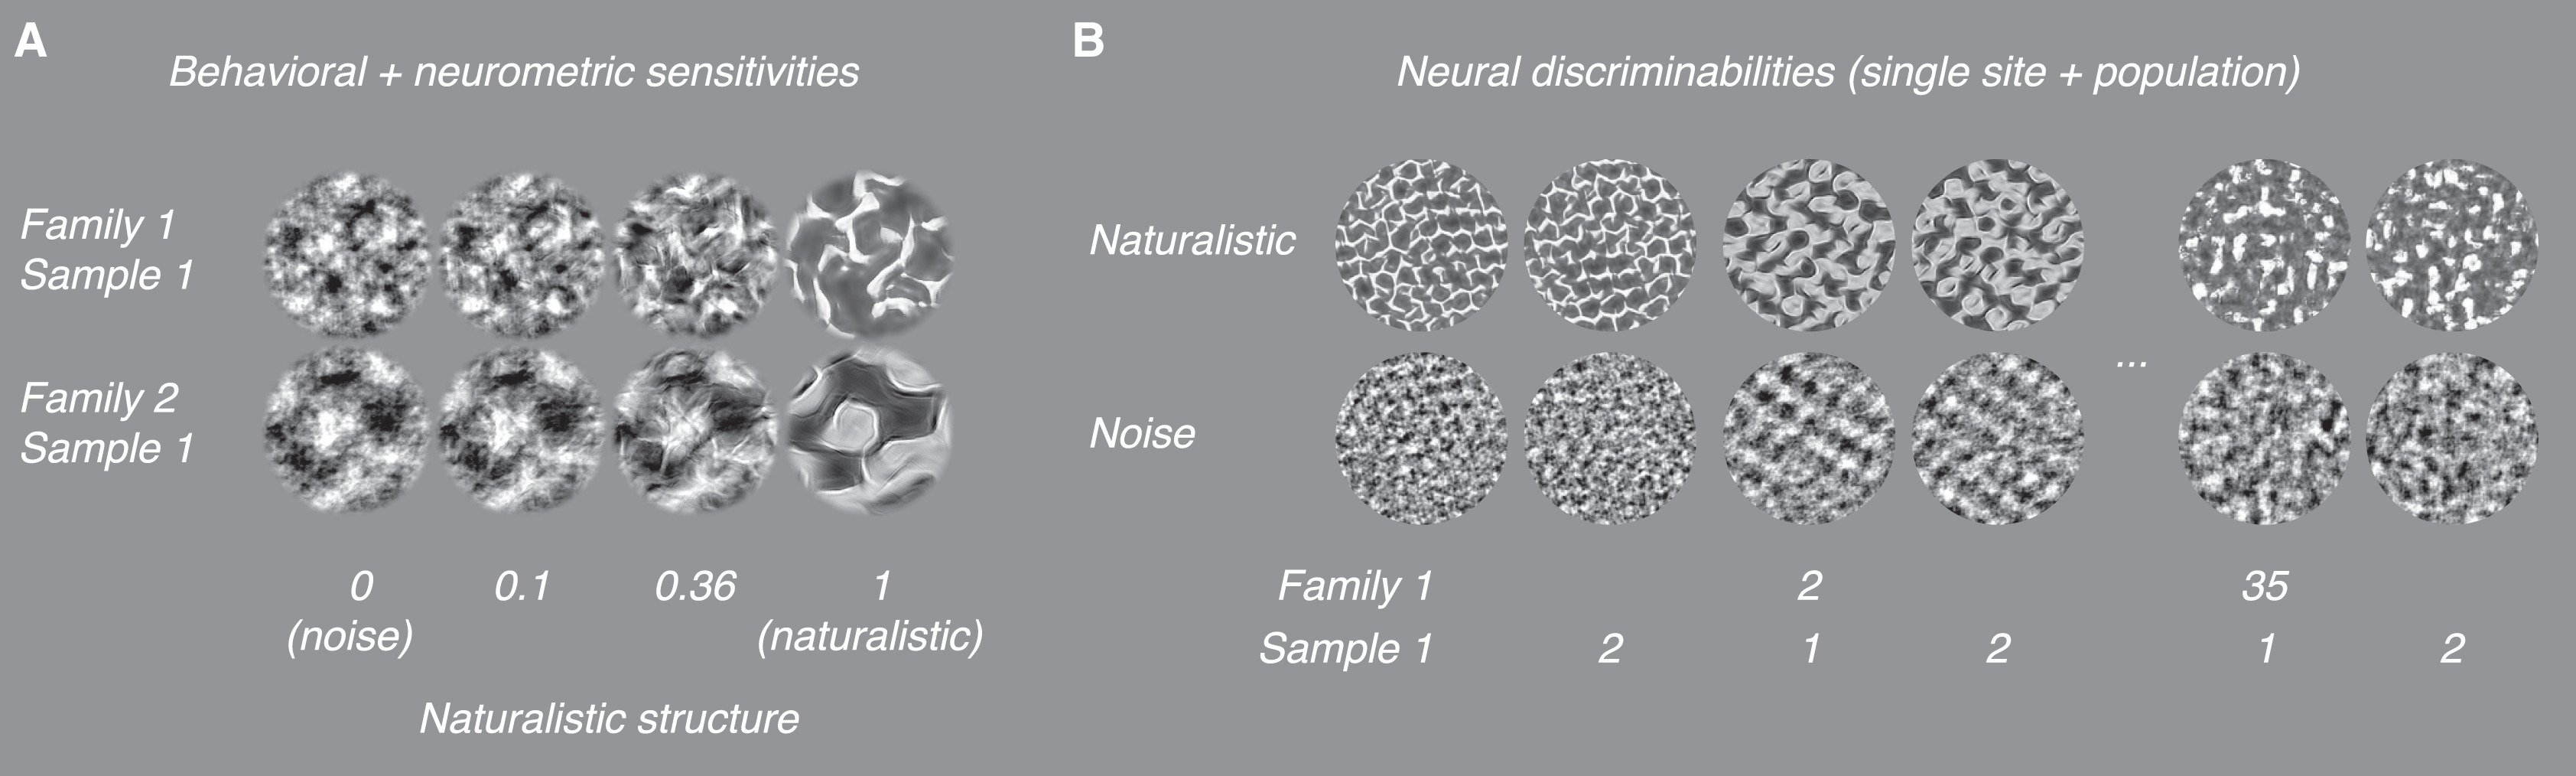
\includegraphics[width=0.9\linewidth,height=\textheight,keepaspectratio]{../img/lee2024-fig01.jpg}

}

\caption{\label{fig-textures}(A) Examples of samples generated with
varying levels of naturalistic structure. (B) Families of samples
generated from different seed images.}

\end{figure}%

\subsection{Passive fixation
recording}\label{passive-fixation-recording}

Lee et al.~recorded from 6 monkeys, each implanted with two 96-site Utah
arrays. Within a session, there were 6 repetitions of each of the
\(35 \times 15 \times 2 = 1050\) unique images, presented in blocks of 8
images (100 ms on, 100 ms off). The provided files aggregate recordings
by region, with the number of sites per region in Table~\ref{tbl-sites}.
For each of V1, V2, V4, and IT, there is at least one 96-electrode Utah
array. The published per-session data reflects simultaneously recorded
sites.

On M1, one array sat on the border between V1 and V2. For M3, the
authors could not reliably determine the location and labeled the region
as the foveal confluence (FC) of V1, V2 and V4, which I removed from my
analyses. Lee et al.~implanted IT arrays twice in M6, with the recording
at 221 weeks taken from the second implantation.

\begin{longtable}[]{@{}llllll@{}}
\caption{The array number is arbitrary. Monkey ID is in
parentheses.}\label{tbl-sites}\tabularnewline
\toprule\noalign{}
Region & Array 1 & Array 2 & Array 3 & Array 4 & Total \\
\midrule\noalign{}
\endfirsthead
\toprule\noalign{}
Region & Array 1 & Array 2 & Array 3 & Array 4 & Total \\
\midrule\noalign{}
\endhead
\bottomrule\noalign{}
\endlastfoot
V1 & 61 (M1) & 96 (M6) & & & 157 \\
V2 & 35 (M1) & 96 (M2) & & & 131 \\
V4 & 96 (M1) & 96 (M2) & 96 (M8) & & 288 \\
IT & 96 (M3) & 96 (M6) & 96 (M6) & 96 (M7) & 384 \\
\end{longtable}

\subsection{Behavioral discrimination between noisy and naturalistic
textures}\label{behavioral-discrimination-between-noisy-and-naturalistic-textures}

In addition to passive fixation recordings, Lee et al.~also measured
behavioral sensitivities with a four-choice oddity task. Monkeys were
shown 3 noisy distractors and 1 naturalistic target, with all four
images produced from the same family. The noisy distractors were unique
samples, i.e., not replicates of the same noisy image. The strength of
naturalistic structure in the target could be modified from 0
(statistically matched to noisy texture) to 1 (fully matches the
naturalistic structure statistics of the seed image). Of the 35 texture
families presented in passive fixation recordings, samples from only
five families were used in the behavioral task. The family IDs in the
behavioral task are included in the public MATLAB code. M8 only
underwent passive fixation recording and did not perform the four-choice
oddity task. M1, M2, and M3 performed the behavioral task prior to
recording while M6 and M7 performed the task after.

\section{References}\label{references}

\phantomsection\label{refs}
\begin{CSLReferences}{0}{1}
\bibitem[\citeproctext]{ref-lee_developmentally_2024}
\CSLLeftMargin{1. }%
\CSLRightInline{Gerick M. Lee, C. L. Rodríguez Deliz, Brittany N.
Bushnell, Najib J. Majaj, J. Anthony Movshon, Lynne Kiorpes.
Developmentally stable representations of naturalistic image structure
in macaque visual cortex. Cell Reports. 2024 Aug 27;43(8).
doi:\href{https://doi.org/10.1016/j.celrep.2024.114534}{10.1016/j.celrep.2024.114534}}

\bibitem[\citeproctext]{ref-ziemba_selectivity_2016}
\CSLLeftMargin{2. }%
\CSLRightInline{Corey M. Ziemba, Jeremy Freeman, J. Anthony Movshon,
Eero P. Simoncelli. Selectivity and tolerance for visual texture in
macaque V2. Proc Natl Acad Sci USA. 2016 May 31;113(22).
doi:\href{https://doi.org/10.1073/pnas.1510847113}{10.1073/pnas.1510847113}}

\bibitem[\citeproctext]{ref-okazawa_image_2015}
\CSLLeftMargin{3. }%
\CSLRightInline{Gouki Okazawa, Satohiro Tajima, Hidehiko Komatsu. Image
statistics underlying natural texture selectivity of neurons in macaque
V4. Proceedings of the National Academy of Sciences. 2015 Jan
27;112(4):E351--60.
doi:\href{https://doi.org/10.1073/pnas.1415146112}{10.1073/pnas.1415146112}}

\bibitem[\citeproctext]{ref-okazawa_gradual_2017}
\CSLLeftMargin{4. }%
\CSLRightInline{Gouki Okazawa, Satohiro Tajima, Hidehiko Komatsu.
Gradual development of visual texture-selective properties between
macaque areas V2 and V4. Cereb Cortex. 2017 Oct 1;27(10):4867--80.
doi:\href{https://doi.org/10.1093/cercor/bhw282}{10.1093/cercor/bhw282}}

\bibitem[\citeproctext]{ref-freeman_functional_2013}
\CSLLeftMargin{5. }%
\CSLRightInline{Jeremy Freeman, Corey M. Ziemba, David J. Heeger, Eero
P. Simoncelli, J. Anthony Movshon. A functional and perceptual signature
of the second visual area in primates. Nat Neurosci. 2013
Jul;16(7):974--81.
doi:\href{https://doi.org/10.1038/nn.3402}{10.1038/nn.3402}}

\bibitem[\citeproctext]{ref-lee_emergence_2025}
\CSLLeftMargin{6. }%
\CSLRightInline{Gerick M. Lee, Najib J. Majaj, C. L. Rodríguez Deliz,
Lynne Kiorpes, J. Anthony Movshon. Emergence of a contrast-invariant
representation of naturalistic texture in macaque visual cortex.
Proceedings of the National Academy of Sciences. 2025 Dec
2;122(48):e2501437122.
doi:\href{https://doi.org/10.1073/pnas.2501437122}{10.1073/pnas.2501437122}}

\bibitem[\citeproctext]{ref-portilla_parametric_2000}
\CSLLeftMargin{7. }%
\CSLRightInline{Javier Portilla, Eero P. Simoncelli. A parametric
texture model based on joint statistics of complex wavelet coefficients.
International Journal of Computer Vision. 2000 Oct 1;40(1):49--70.
doi:\href{https://doi.org/10.1023/A:1026553619983}{10.1023/A:1026553619983}}

\end{CSLReferences}




\end{document}
